\documentclass[14pt]{extreport}
\usepackage{gost}

%Тут можно вставить дополнительные пакеты

\begin{document}
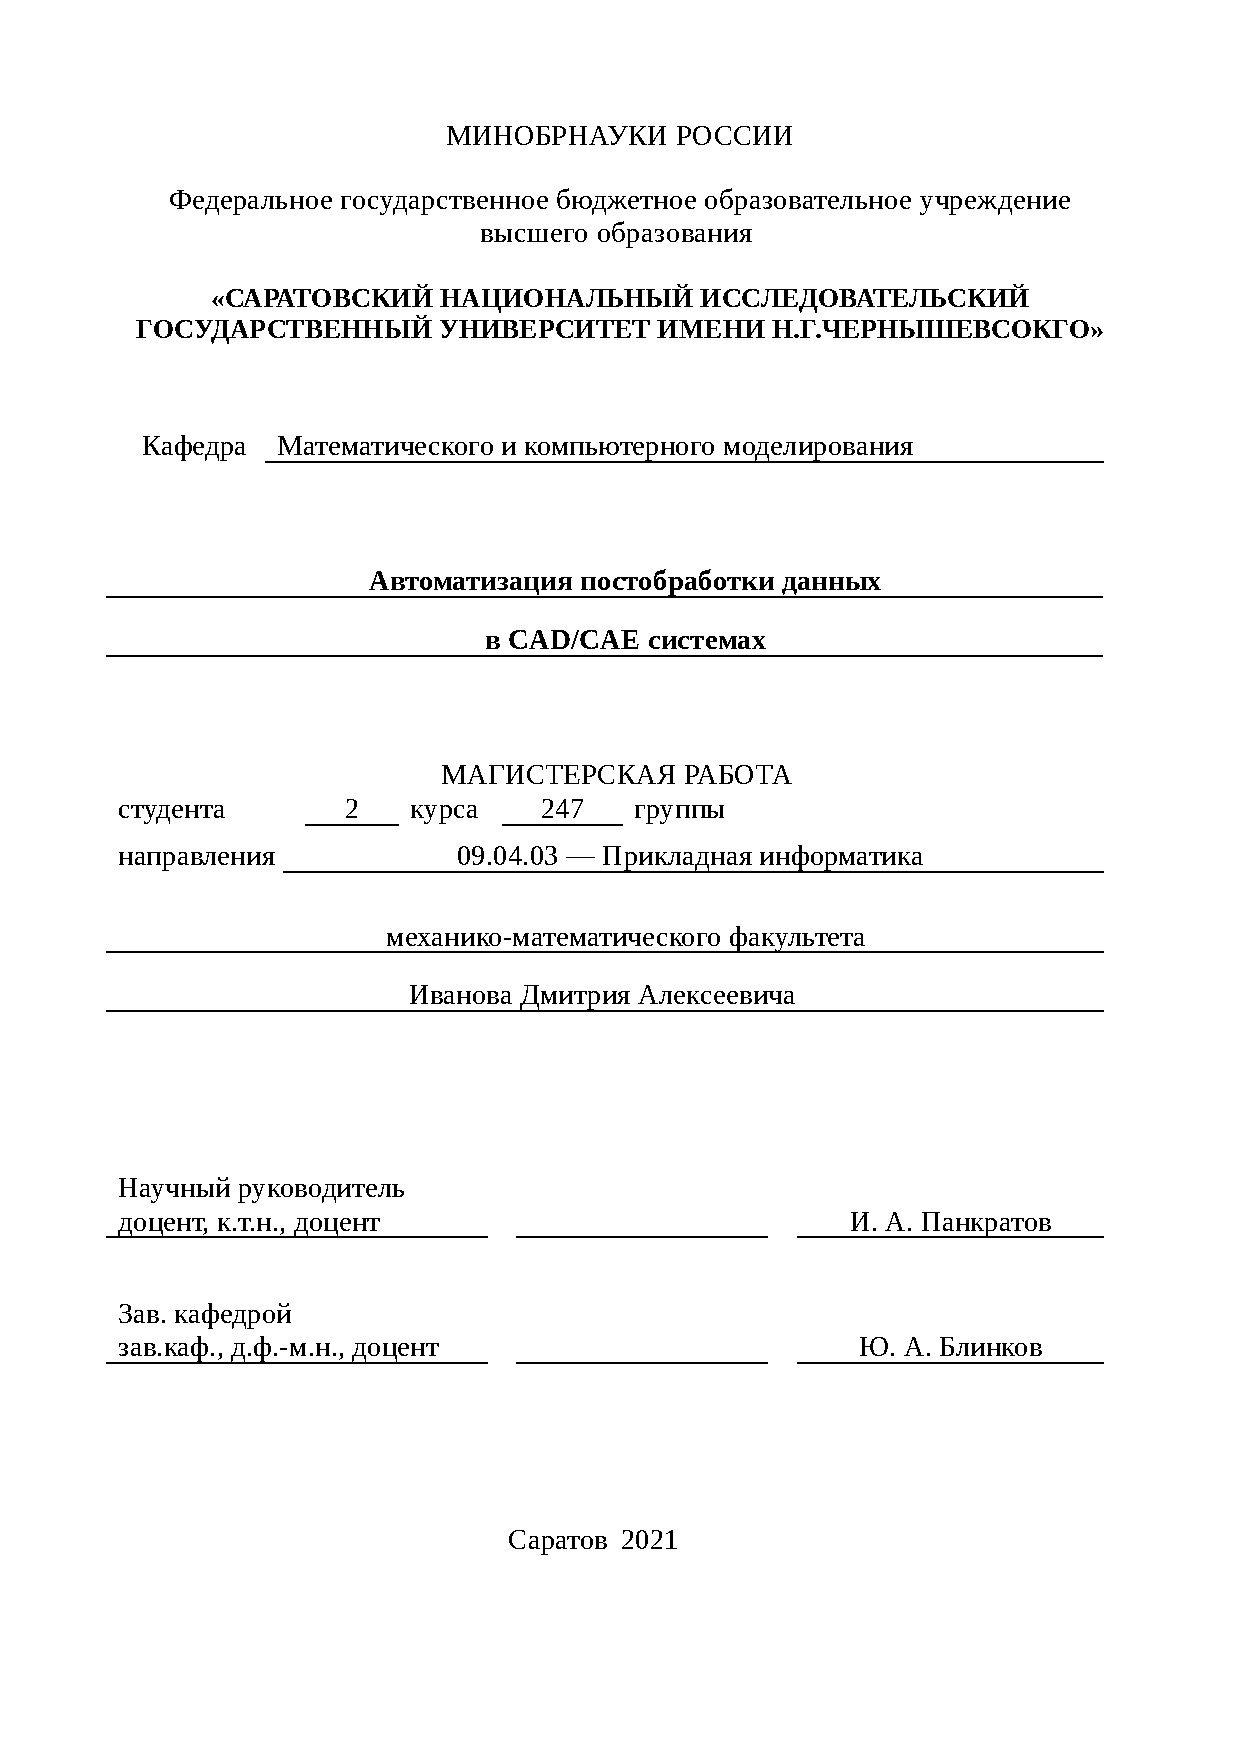
\includepdf[pages={1}]{titulCourse.pdf}

% ТЕМА: Анализ экспериментальных данных с помощью NoSQL

\tableofcontents

\intro
При обработке экспериментальных данных, полученных в результате математического моделирования физических процессов в CAD/CAE системах, особенно, когда проводиться, например, серия экспериментов, в которых входные данные незначительно изменяются часто порождается большой объем результатов, надлежащих анализу или иными словами -- пост-обработке. Причем, зачастую для анализа с полученными мало различающимися данным необходимо провести однотипные манипуляции. Учитывая все выше сказанное, становится ясна необходимость автоматизации такого процесса пост-обработки данных. 

В курсовой работе будет спроектирована информационная система позволяющая упростить процесс анализа полученных экспериментальных данных. Для автоматизации будет использован язык программирования Python, для хранения результатов -- NoSQL подход, а конкретно СУБД MongoDB. 

Таким образом целью данной курсовой работы является проектирование информационной системы, автоматизирующей рутинные операции анализа экспериментальных данных.
Задачи:
\begin{itemize}
\item Кратко рассмотреть CAD/CAE систему -- OpenFOAM и ParaView.
\item Рассмотреть существующие решения по данной тематике.
\item Спроектировать UML-диаграммы для описания информационной системы.
\end{itemize}

\chapter{Краткая информация об OpenFOAM и ParaView}
\section{OpenFOAM}
OpenFOAM (англ. Open Source Field Operation And Manipulation CFD ToolBox) — открытая интегрируемая платформа для численного моделирования задач механики сплошных сред. ~\cite{OpenfoamWiki}

Это пакет программ распространяемых свободно под лицензией GNU GPL, позволяющей решать задачи механики сплошных сред, в частности: 
\begin{itemize}
\item Прочностные расчеты;
\item Гидродинамика ньютоновских и неньютоновских вязких жидкостей как в несжимаемом, \item так и сжимаемом приближении с учётом конвективного теплообмена и действием сил гравитации. Для моделирования турбулентных течений возможно использование RANS-моделей, LES- и DNS-методов. Возможно решение дозвуковых, околозвуковых и сверхзвуковых задач;
Задачи теплопроводности в твёрдом теле;
\item Многофазные задачи, в том числе с описанием химических реакций компонент потока;
\item Задачи, связанные с деформацией расчётной сетки;
\item Сопряжённые задачи;
\item Некоторые другие задачи, при математической постановке которых требуется решение дифференциальных уравнений в частных производных в условиях сложной геометрии среды;
\end{itemize}

В основе кода лежит набор библиотек, предоставляющих инструменты для решения систем дифференциальных уравнений в частных производных как в пространстве, так и во времени. Рабочим языком кода является C++. OpenFOAM состоит из приблизительно 250 программ основанных на более чем 100 библиотеках. Каждое приложения выполняет свою конкретную задачу в рамках процесса расчета. Этапы работы представленные в соответствии с рисунком ~\ref{fig}.

\begin{figure}[H]
\centerline{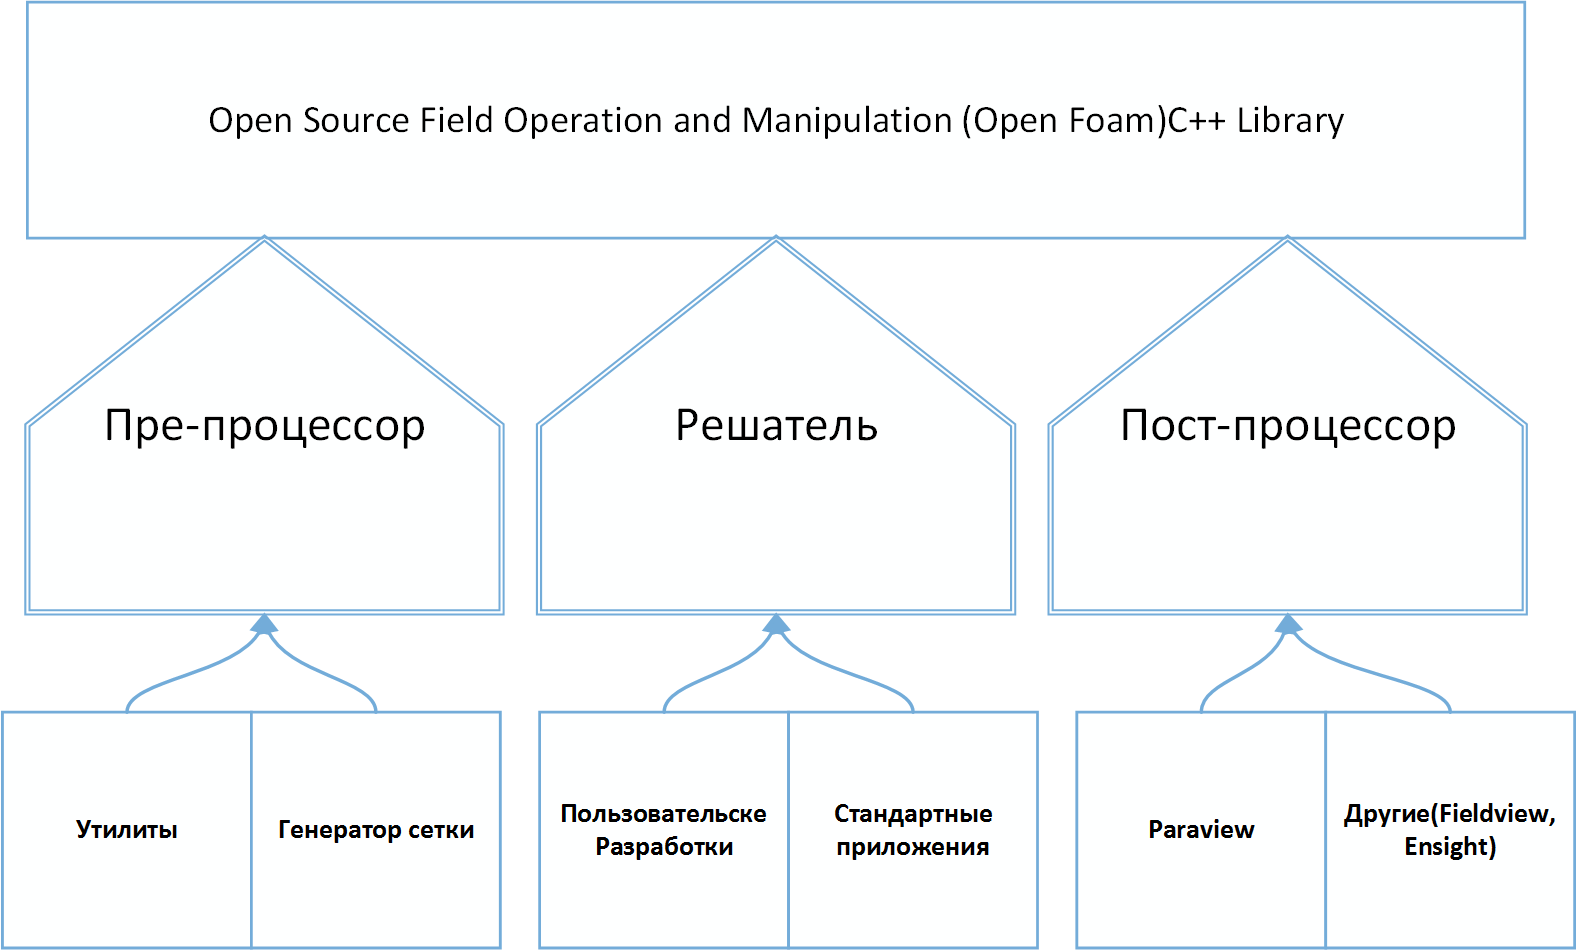
\includegraphics[width=1.0\linewidth]{OFScheme}}
\caption{Утилиты и программы входящие в пакет OpenFOAM, сгруппированные по этапам работы с расчетом.}
\label{fig1}
\end{figure}

Работа с программой делится на три этапа:
\begin{enumerate}
\item Пре-процессинг;
\item Решение;
\item Пост-процессинг.
\end{enumerate}

На этапе пре-процессинга в специальных файлах задаются входные данные для рассчета примера, такие как: начальное время, конечное время, шаг и так далее. Также параметры для хранения решения: время, формат, тип сжатия. Также в препроцессинг включены настройки выбора различных схем рассчета, котоыре влияют на точность и стабильность решения. После этого отдельно генерируется расчетная область (сетка), которая вполседствии может быть обработана различными утилитами ~\cite{OpenfoamUserGuide}. Затем запускается решатель, который производит расчет. На этапе пост-процессинга полученные данные представляются в виде графиков. Также используются некоторые утилиты, например для конвертации из внутреннего формата OpenFOAM в широко используемый формат vtk.

\section{ParaView}
ParaView -- открытый графический кросс-платформенный пакет для интерактивной визуализации в исследовательских целях, разрабатываемый Национальной Лабораторией Сандиа, компанией Kitware и Национальной Лабораторией Лос-Аламоса \cite{ParaviewAbout}.

Пакет ParaView предоставляет пользователю возможности интерактивной визуализации и исследования больших массивов данных для качественного и количественного анализа.

Пакет может быть использован на компьютерах с операционными системами Windows, Linux, Mac OS X.

При разработке авторы придерживаются следующих целей:
\begin{itemize}
\item Открытость, кросс-платформенность — в пакете используются только открытые, мульти-платформенные технологии для визуализации данных.
\item Поддержка различных, в том числе, гетерогенных вычислительных систем.
\item Создание гибкого, интуитивного пользовательского интерфейса.
\end{itemize}

Таким образом, пакет ParaView во многом является скорее технологией обработки, чем всего лишь программным средством ~\cite{ParaviewWiki}.

Одни из основных возможностей пакета:
\begin{itemize}
\item Визуализация расчетных областей.
\item Визуализация полей (давление, скорость, температура, смещения и прочее).
\item Построение срезов областей как плоскостью, так и заданной функцией.
\item Построение изо-поверхностей.
\item Построение векторных полей и линий тока.
\item Позволяет показывать динамику развития протекающего процесса, отображая анимацию. 
\end{itemize}

Основной формат данных ParaView -- VTK, но пакет также содержит драйверы для работы с форматом OpenFOAM и поставляется вместе с дистрибутивом пакета. 

Работа с Paraview может осуществляться как в интерактивном, так и пакетном режиме.
Приложение 

ParaView также предлагает богатый и мощный програмный интерфейс на языке Python. Это позволяет пользователям автоматизировать обработку своих данных и использовать возможности, так называемого, набора инструментов визуализации -- Visualization Tool Kit (VTK) ~\cite{ParaviewAndPython}.

\chapter{Обзор существующих решений}
Рассматриваемая в данной курсовой работе информационная система должна выполнять пост-обработку данных, полученных в результате численно эксперимента в пакете OpenFOAM, делая упор на автоматизацию функций для работы с серией данных. Рассмотрим доступные приложение осуществляющие автоматизацию рутинных функций в рамках пакета OpenFOAM.
\section{HELYX OS}
HELYX-OS - это графический пользовательский интерфейс с открытым исходным кодом, разработанный компанией ENGYS для работы со стандартными библиотеками OpenFOAM, предоставляемыми OpenFOAM Foundation и ESI-OpenCFD. Приложение предназначено для академического использования и работы с CFD начального уровня. Распространяется в соответствии с GNU General Public License ~\cite{Helyx}.

HELYX-OS предоставляет полностью интерактивную, простую в использовании среду для выполнения всех задач предварительной обработки в процессе CFD, включая создание сетки, определение случая и выполнение решателя.

Существует также версия для корпоративного использования -- CFD HELYX.

Преимущества: 
\begin{itemize}
\item Встроенная поддержка как OpenFOAM, так и OpenFOAM+: возможность загружать существующие кейсы, читая настройки непосредственно из доступных текстовых файлов проекта.
\item Программа доступна на платформах Linux и Windows. Однако версия для Windows платна.
\item Управление утилитой построения сеток snappyHexMesh, включая такие возможности как отображение геометрии и непосредственное построение прямо в окне приложения.
\item Отдельный мониторинг решателя с отслеживанием остатков решения.
\end{itemize}

В корпоративной версии также следует выделить:
\begin{itemize}
\item Высокая масштабируемость.
\item Возможность работы с использованием облачных технологий.
\item Модульность. Возможно расширение в рамках HELYX ADD-ONS, 
\end{itemize}

В соответствии с рисунком ~\ref{fig2} изображен рабочий экран программы.

\begin{figure}[H]
\centerline{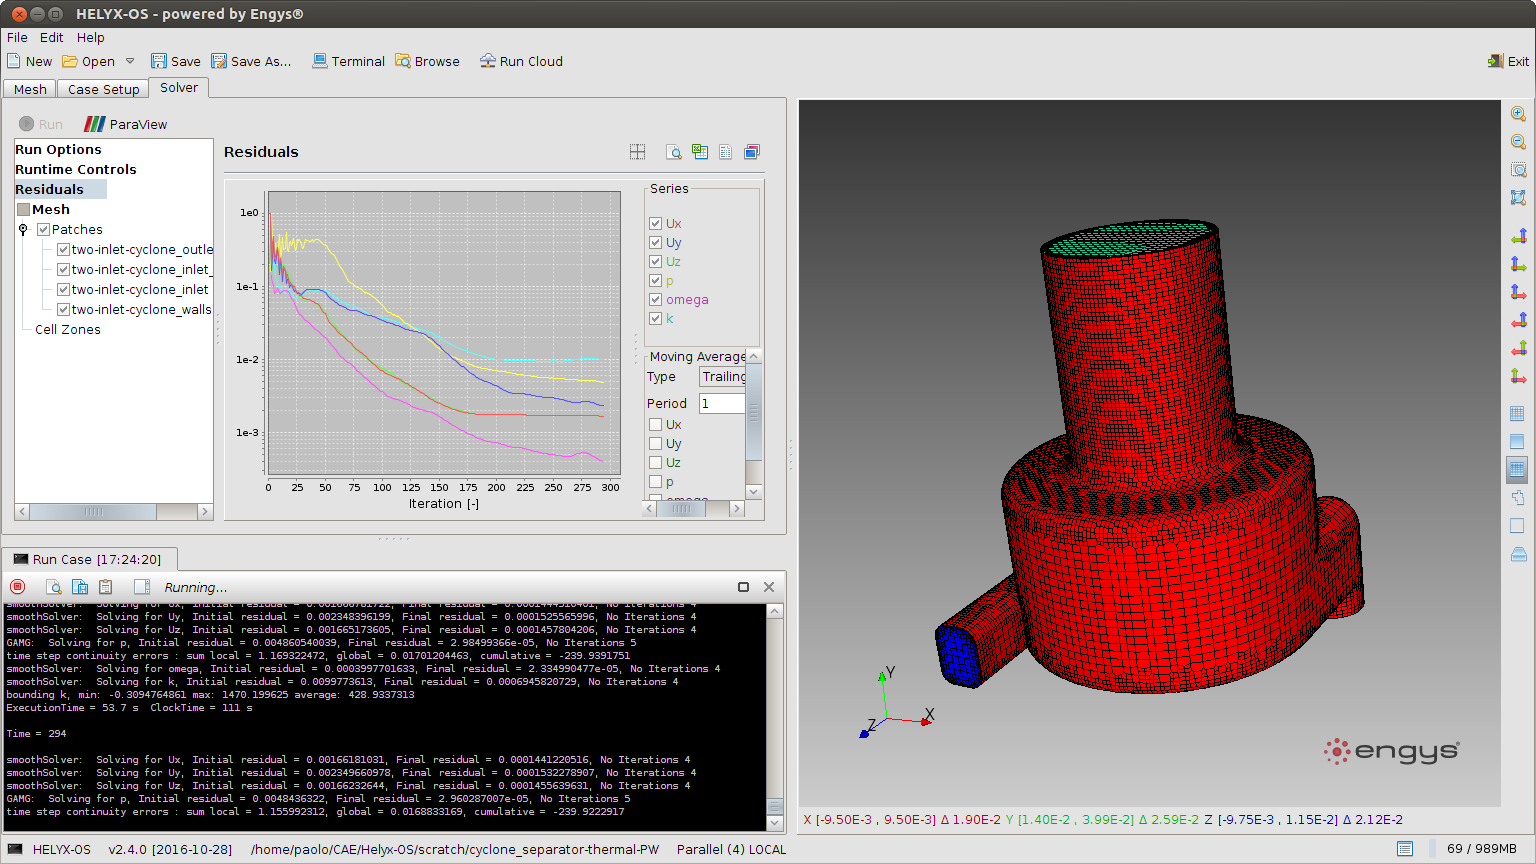
\includegraphics[width=1.0\linewidth]{helyxos}}
\caption{Рабочий экран приложения Helyx OS.}
\label{fig2}
\end{figure}

\section{ANSA}
ANSA - это инструмент пре-процессинга CAE, который предоставляет все необходимые функциональные возможности для построения полной модели, от CAD-данных  до готового к вводу файла решателя, в единой интегрированной среде ~\cite{Ansa}.

Все функции программного обеспечения размещены в интегрированной среде с настраиваемым графическим интерфейсом. Программное обеспечение доступно для всех современных популярных операционных систем в 32-битной и 64-битной архитектуре с использованием многоядерных процессоров. 

Преимущества: 
\begin{itemize}
\item Эффективная обработка данных для сложных структур моделей.
\item Быстрое и качественное моделирование сложных геометрических моделей.
\item Возможность взаимодействия между моделями, созданными для разных решателей.
\item Высокоавтоматизированные процессы и инструменты настройки модели в одной программе.
\item Уменьшены зависящие от пользователя подверженные ошибкам операции.
\item Полное построение модели для многочисленных решателей в одной среде.
\end{itemize}
Рабочий экран приложения представлен в соответствии с рисунком ~/ref{fig3}

\begin{figure}[H]
\centerline{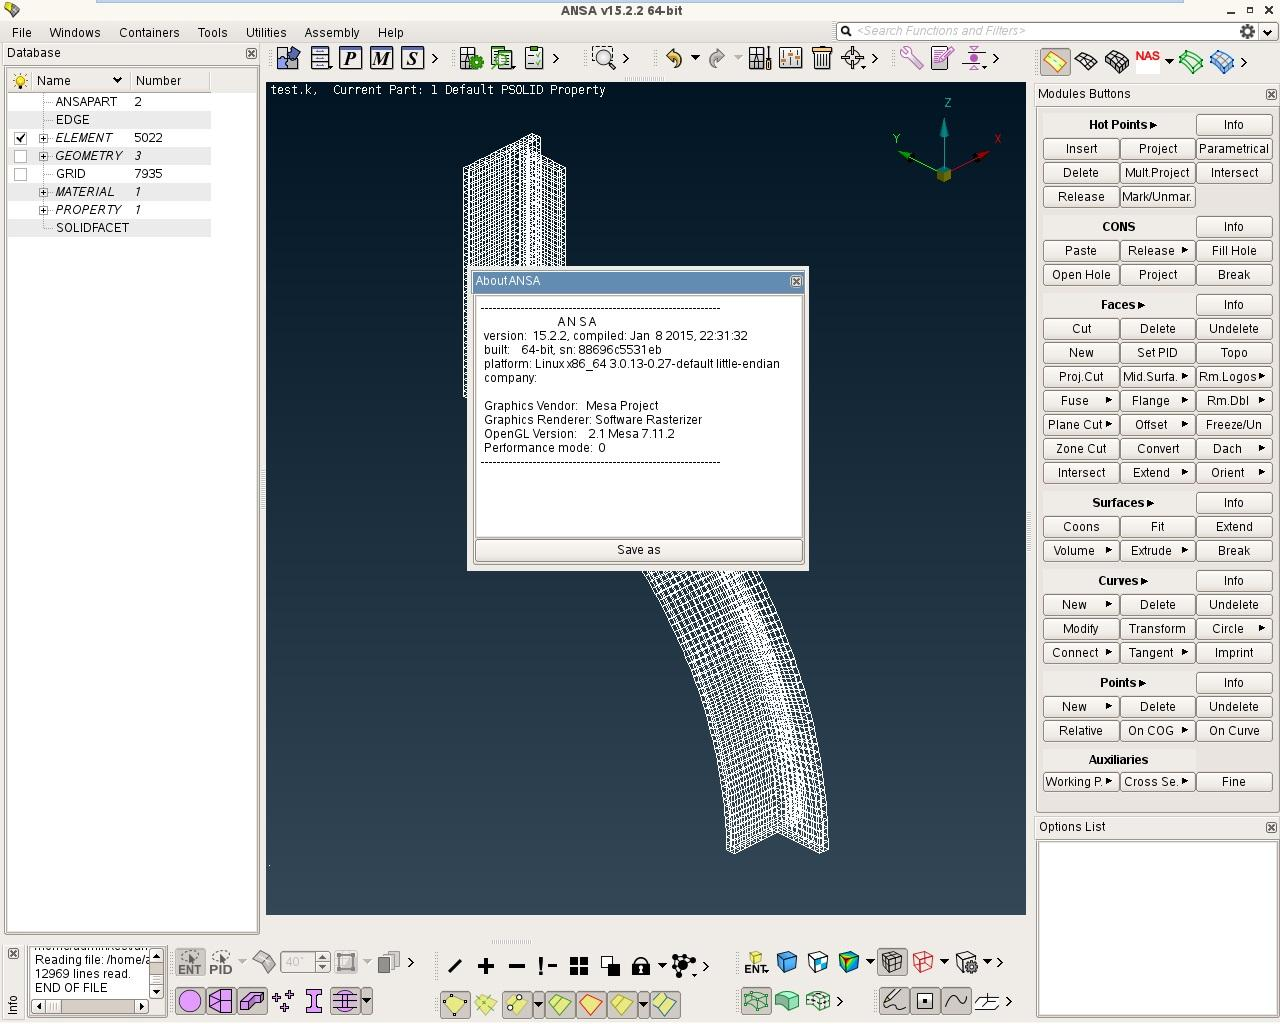
\includegraphics[width=1.0\linewidth]{ansa}}
\caption{Рабочий экран приложения ANSA.}
\label{fig3}
\end{figure}

\section{CastNet}

CastNet упрощает использование технологических решений CAE для решателей с открытым исходным кодом: кроме типичного редактирования текстовых файлов, предоставляется альтернативный способ работы с OpenFOAM на основе графического интерфейса, сохраняя полную совместимость со стандартными выпусками OpenFOAM. В результате рабочий процесс становится достаточно гибким, и пользователь может в любой момент переключаться между настройкой рабочего примера на основе текстового файла и графического интерфейса пользователя.

Вид рабочего экрана приложения представлен в соответствии с рисунком ~\ref{fig4}
\begin{figure}[H]
\centerline{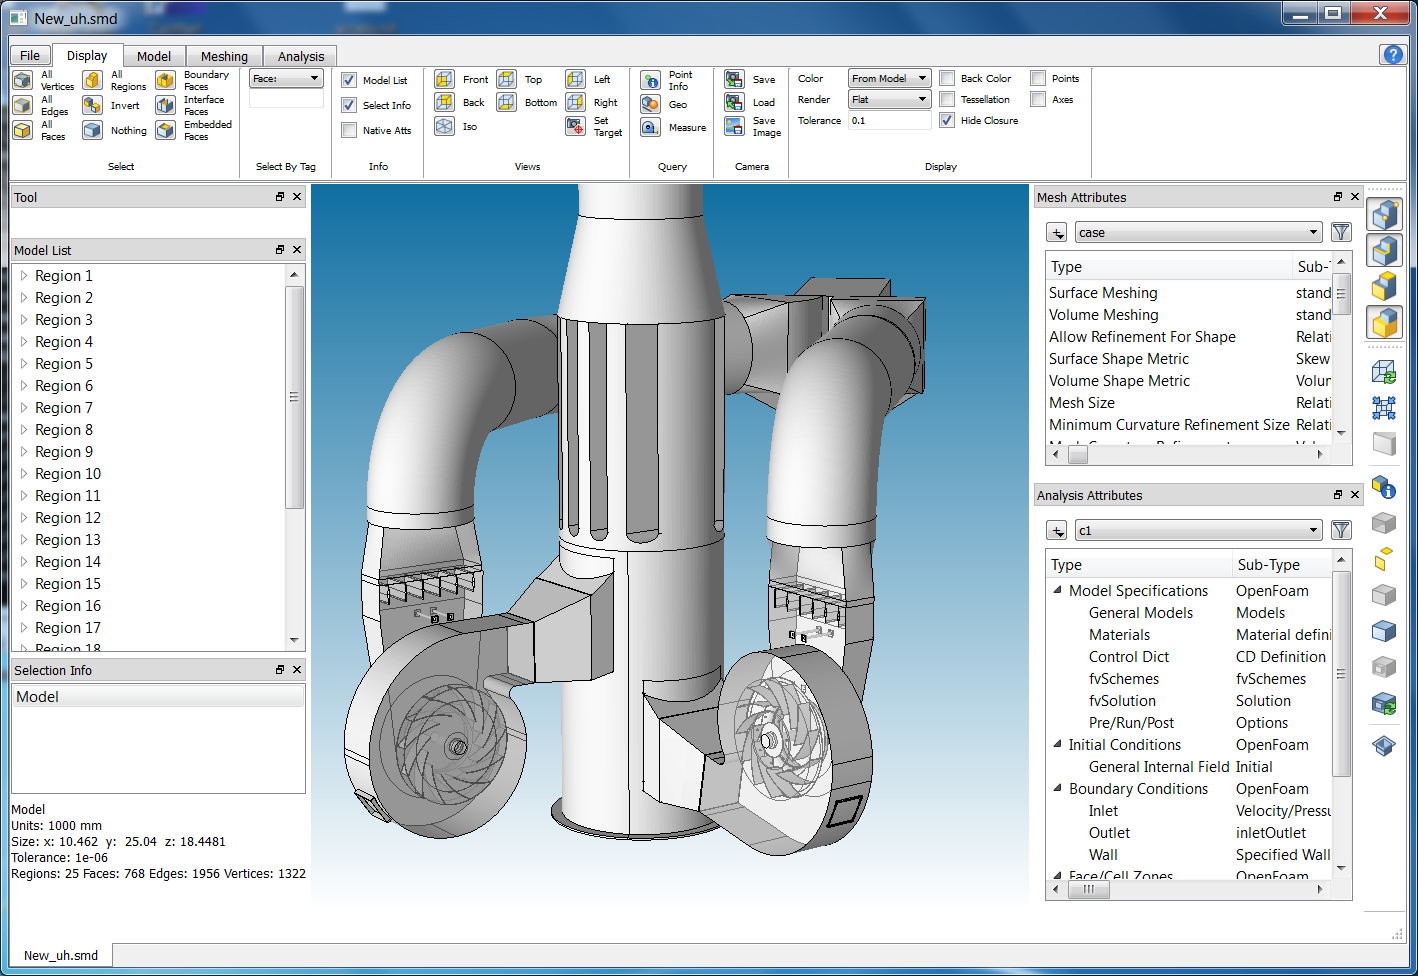
\includegraphics[width=1.0\linewidth]{castnet}}
\caption{Рабочий экран приложения CastNet.}
\label{fig4}
\end{figure}

Ключевые особенности CastNet:
\begin{itemize}
\item Полноценная среда разработки на основе графического интерфейса пользователя, включающая предварительную обработку (создание сетки, настройку примера), мониторинг решения и последующую обработку. Таким образом: доступ к мощным функциям решателя с открытым исходным кодом без редактирования текстовых файлов или необходимости детального изучения структуры ключевых слов OpenFOAM.
\item Кроссплатформенное использование: поддержка гибкой среды для пакета программ OpenFOAM в операционных системах Windows и Linux.
\item Большая библиотека шаблонов, позволяющая легко настраивать пример для более чем 30 решателей OpenFOAM.
\item Больше надежности в отношении результатов моделирования благодаря контролю сходимости.
Разработчики также особо выделяют совместимость со всеми версиями пакета программ OpenFOAM.
\end{itemize}

\chapter{Проектирование информационной системы}
\section{Постановка задачи}
Необходимо спроектировать приложение, которое бы выполняло процесс пост-обработки, то есть строило графики используя экспериментальные данные полученные из пакета программ OpenFOAM. Приложение должно также работать с группами экспериментальных данных, то есть выполнять конкретное действие построения графика, например срез, с группой из разных мало отличающихся кейсов. Программа должна хранить экспериментальные данные и историю операций кейса. Для этого будет использована СУБД MongoDB. Для построения графиков будет использован API ParaView на языке Python. Также должна быть реализована возможность экспорта графиков в файлы.

Для более подробного понимания информационной системы были построены UML-диаграммы. 

\section{Диаграмма прецедентов}
Прецеденты -- это технология определения функциональных требований к системе ~\cite{umlDistilled}. 
Диаграмма прецедентов (use case diagram) предназначена для описания взаимодействия проектируемой системы с любыми внешними или внутренними объектами - пользователями, другими системами и тому подобное.
Основными понятиями при работе с диаграммой вариантов использования являются 
Актор (Actor) -- это роль, которую выполняет пользователь или другая система, при взаимодействии с проектируемой системой.
Вариант использования -- это конечная единица взаимодействия актора и системы. 

Диаграмма вариантов использования представлена в соответствии с рисунком ~\ref{fig5}
\begin{figure}[H]
\centerline{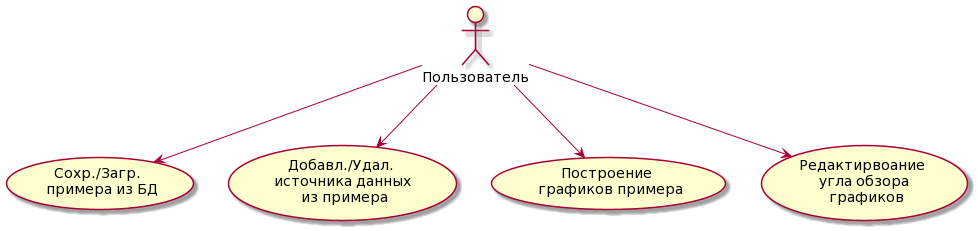
\includegraphics[width=1.0\linewidth]{userCaseDiagram}}
\caption{Диаграмма прецедентов.}
\label{fig5}
\end{figure}

В соответствии с рисунком ~\ref{fig5} представлена базовая функциональность проектируемой программы. Пример или основная сущность программы состоит из списка источников данных. Каждый источник данных -- это результат конкретного численного эксперимента. Таким образом достигается цель -- работа сразу с несколькими источниками данных.   
\section{Диаграмма классов}
Диаграмма классов описывает типы объектов системы и различного рода статические отношения, которые существуют между ними. На диаграммах классов отображаются также свойства классов, операции классов и ограничения, которые накладываются на связи между объектами ~\cite{umlDistilled}.

Для удобства рассмотрения разобьем диаграмму классов на три рисунка. Каждый из которых соответствует определенной решаемой задачи. 

\subsection{Диаграмма, представляющая способ организации экспериментальных данных}

В соответствии с рисунком ~\ref{fig6} представленная диаграмма классов, иллюстрирует способ организации экспериментальных данных в приложении. 

Класс Data -- ООП представление данных полученных в результате численного эксперимента в OpenFOAM. Он неразрывно связан с классом-оберткой ExpData -- в нем экземпляру присваивается идентификатор и хранится другая служебная информация необходимая программе. 

\begin{figure}[H]
\centerline{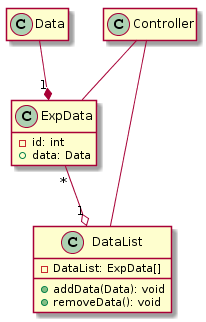
\includegraphics[height=1.0\linewidth]{classDiagram_Data-Controller}}
\caption{Диаграмма классов, представляющая способ организации экспериментальных данных.}
\label{fig6}
\end{figure}

Так как проектируемое приложение должно работать с некоторым набором экспериментальных данных, то бы введен класс DataList, который, как видно в соответствии с рисунком ~\ref{fig6}, содержит список этих данных. Данный класс вступает в качестве поля класса Сase. Это класс, содержащий основную информацию о текущей сессии приложения, будет рассмотрен чуть более подробнее далее. 

Класс ExpData и DataList ассоциирован с классом Controller, где происходит их инстанцирование и инициализация. Класс Controller объединяет работу частей модели программы и связывает их с графическим интерфейсом пользователя. 

\subsection{Диаграмма для работы с базой данных и чтения экспериментальных данных}
В соответствии с рисунком ~\ref{fig7} представленная диаграмма классов, иллюстрирует работу приложения с базой данных и чтение экспериментальных данных.

Статический класс ApplicationUtils реализует чтение экспериментальных данных и настроек приложения из файла. Класс DTO (Data Transfer Object) используется в качестве промежуточной сущности для валидации данных.

Класс Database -- используется для установления соединения и работы с базой данных. Данный класс будет реализован при помощи паттерна проектирования синглтон (Singleton). Данный паттерн гарантирует, что у класса есть только один экземпляр, и предоставляет к нему глобальную точку доступа ~\cite{oop}. Такой подход дает позволяет только один раз при первом обращении произвести ресурсоемкую операцию установления соединения с базой данных, а после каждый раз при последующих обращениях возвращать уже созданный экземпляр класса. Получение различных сущностей из базы данных будет осуществляться при помощи класса DAO (Data Access Object). Этот прием позволит не передавать лишнюю информацию в модель приложения.

\begin{figure}[H]
\centerline{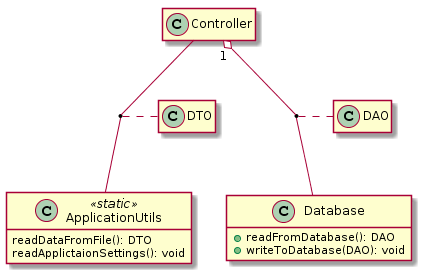
\includegraphics[width=1.0 \linewidth]{classDiagram_DB-AppUtils-Controller}}
\caption{Диаграмма классов для работы с базой данных и чтения экспериментальных данных.}
\label{fig7}
\end{figure}

\subsection{Диаграмма классов для выполнения операций над графиками}
В соответствии с рисунком ~\ref{fig8} представленная диаграмма классов иллюстрирует организацию классов, реализующих операции над графиками.

Класс Case хранит необходимую информацию о текущей сессии, в частности загруженные источники данных (класс ExpData) и историю операций -- построенные графики. В классе OperationHistory непосредственно хранится информация о построенных графиках. 

\begin{figure}[H]
\centerline{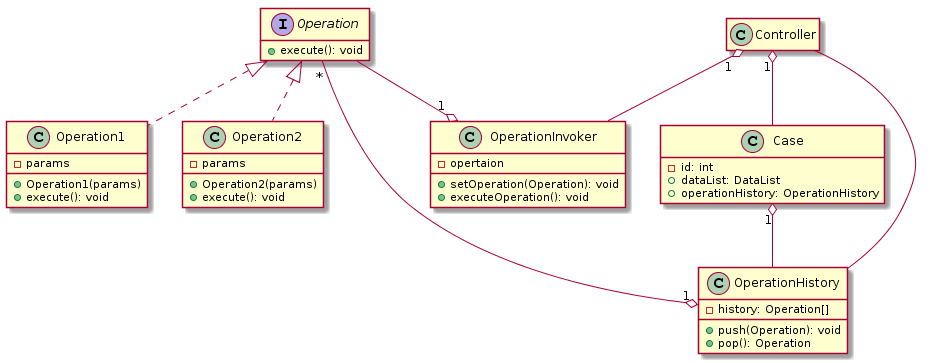
\includegraphics[width=1.1 \linewidth]{classDiagram_Case-Operaion-Controller}}
\caption{Диаграмма классов для выполнения операций над графиками.}
\label{fig8}
\end{figure}

В целом, существуют разные виды графиков, а пользователем может быть последовательно запланировано несколько различных операций поэтому представляется разумным для организации этой функциональности применить паттерн проектирования команда (command или action).

Команда -- это поведенческий паттерн проектирования, который превращает запросы в объекты, позволяя передавать их как аргументы при вызове методов, ставить запросы в очередь, логировать их, а также поддерживать отмену операций \cite{pattern}. В случае данной информационной системы в роли команды выступает операция построения графика или иная связанная с этим операция.

Структура паттерна следующая: 
\begin{itemize}
\item Класс OperationInvoker хранит ссылку на объект операции и обращается к нему, когда нужно выполнить какое-то действие. OperationInvoker работает с операциями только через их общий интерфейс. Он не знает, какую конкретно опрециб использует, так как получает готовый объект операции от класса Controller.

\item Operation описывает общий для всех конкретных операций интерфейс. Здесь задан метод execute для запуска операции.

\item Конкретные операции, это классы Operation1 и Operation2, представленные в соответствии с рисунком ~\ref{fig8}, реализуют различные запросы, следуя общему интерфейсу операций. У них реализованы методы execute, а конструктор принимает параметры (params), таким образом предоставляя возможность сделать операции неизменяемыми.

\item В рамках данного паттерна класс Controller создаёт объекты конкретных операций, передавая в них все необходимые параметры.
\end{itemize}

\section{Диаграмма последовательностей}
Диаграммы взаимодействия (interaction diagrams) описывают взаимодействие групп объектов в различных условиях их поведения. UML определяет диаграммы взаимодействия нескольких типов, из которых наиболее употребительными являются диаграммы последовательности (sequence diagram)~\cite{umlDistilled}.

На диаграмме последовательностей отображаются системные события для одного
сценария некоторого прецедента. Поэтому сама диаграмма строится на основе описания
прецедента ~\cite{umlApplying}. 

Если прецедент отвечает на вопрос <<Что делает актор?>>, то последовательность отвечает на вопрос <<Как работает система при выполнении данного прецедента?>>.
Каждый прецедент может содержать несколько диаграмм последовательностей, на тот случай, если они описывают несколько альтернативных вариантов развития событий.

Диаграмма последовательностей будет построена только для прецедента <<Построение графиков примера>>, <<Сохранение примера в базу данных>>, <<Добавление источника 
данных>>.

В соответствии с рисунком ~\ref{fig9} представлена диаграмма последовательностей для прецедента <<Построение графиков примера>>.

\begin{figure}[H]
\centerline{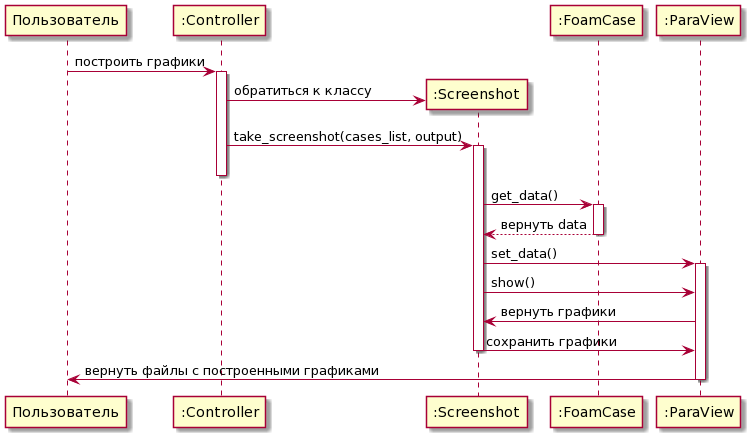
\includegraphics[width=1.1 \linewidth]{sequenceDiagram_graphs}}
\caption{Диаграмма последовательностей для прецедента <<Построение графиков примера>>.}
\label{fig9}
\end{figure}

В соответствии с рисунком ~\ref{fig10} представлена диаграмма последовательностей для прецедента <<Построение графиков примера>>.

\begin{figure}[H]
\centerline{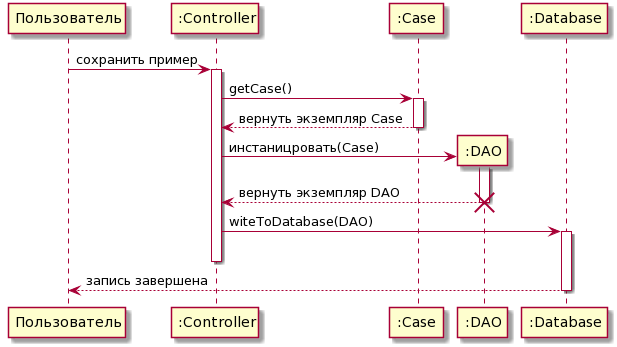
\includegraphics[width=1.1 \linewidth]{sequenceDiagram_saveToDB}}
\caption{Диаграмма последовательностей для прецедента <<Сохранение примера в базу данных>>.}
\label{fig10}
\end{figure}

В соответствии с рисунком ~\ref{fig11} представлена диаграмма последовательностей для прецедента <<Добавление источника данных>>.

\begin{figure}[H]
\centerline{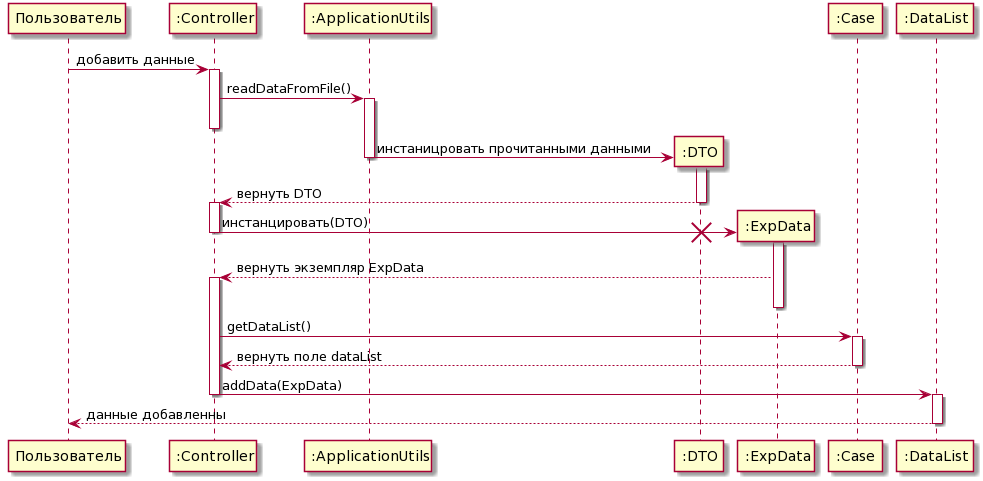
\includegraphics[width=1.1 \linewidth]{sequenceDiagram_addData}}
\caption{Диаграмма последовательностей для прецедента <<Добавление источника 
данных>>.}
\label{fig11}
\end{figure}

\conclusions
В данной работе кратко рассмотрен пакет программ для численного моделирования OpenFOAM, приложения для пост-процессинга ParaView. Была поставлена задача проектирования информационной системы. Выполнена первая итерация проектирования, необходимая для начала написания приложения, в частности построены UML-диаграммы прецедентов, классов, последовательностей. Также были рассмотрены существующие на данным момент решение по пост-обработки экспериментальных данных.

Таким образом, задачи данной работы были выполнены и, следовательно, поставленная цель была достигнута. 



% Оформляем библиографию в соответствии с ГОСТ 7.0.5
\bibliographystyle{ugost2008}
% если хотим включить все источники из библиографии даже не имеющие ссылки из текта
% \nocite{*}
% файл с библиографией
\bibliography{biblio.bib}

% \Appendix % Приложения

\end{document}
